\begin{figure*}[ht]
	\setlength{\abovecaptionskip}{0pt}
	\setlength{\belowcaptionskip}{-10pt}
	\centering
	\subfigure[Web Search.]{
		\begin{minipage}[b]{0.46\textwidth}
			% height=1.7in, width=3in
			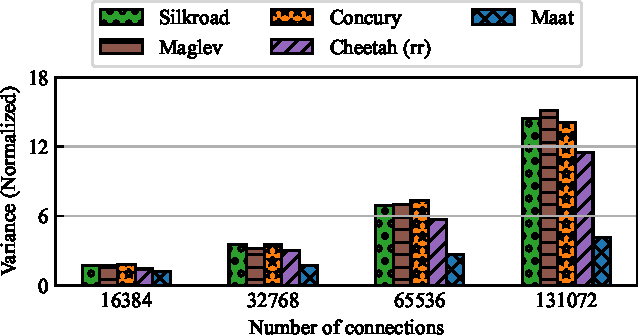
\includegraphics[width=1\linewidth]{experiment/3maatvarianceschemewb.pdf}
		\end{minipage}
		\label{8.1}
	}
	\subfigure[Data Mining.]{
		\begin{minipage}[b]{0.46\textwidth}
			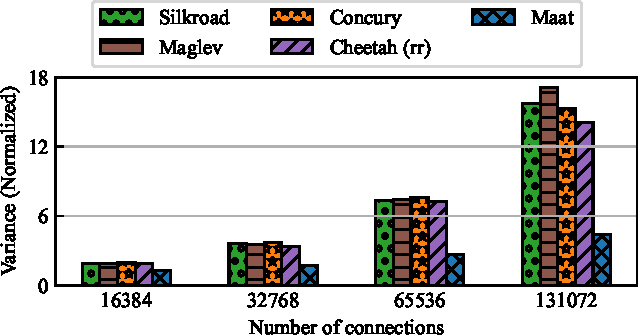
\includegraphics[width=1\linewidth]{experiment/3maatvarianceschemedm.pdf}
		\end{minipage}
		\label{8.2}
	}
	\vspace{0pt}
	\caption{Variance among servers’ load of various L4 LB schemes for increasing connections.}
	\label{8}
\end{figure*}

\begin{figure*}[ht]
	\setlength{\abovecaptionskip}{0pt}
	\setlength{\belowcaptionskip}{-10pt}
	\centering
	\subfigure[Web Search.]{
		\begin{minipage}[b]{0.46\textwidth}
			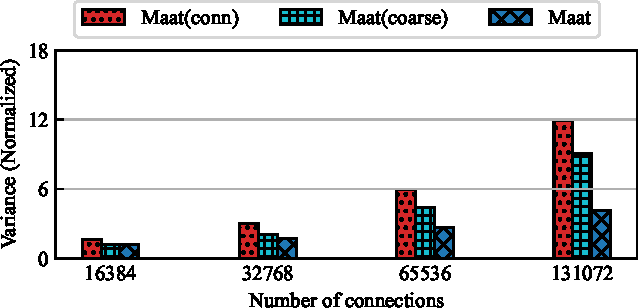
\includegraphics[width=1\linewidth]{experiment/4maatvariancegranwb.pdf}
		\end{minipage}
		\label{9.1}
	}
	\subfigure[Data Mining.]{
		\begin{minipage}[b]{0.46\textwidth}
			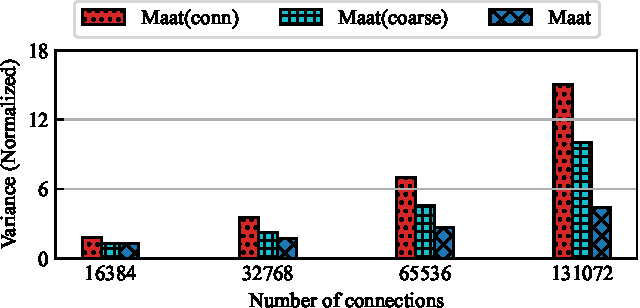
\includegraphics[width=1\linewidth]{experiment/4maatvariancegrandm.pdf}
		\end{minipage}
		\label{9.2}
	}
	\vspace{0pt}
	\caption{Variance among servers’ load of different collect traffic status methods for increasing connections.}
	\label{9}
\end{figure*}

\section{IMPLEMENTATION AND EVALUATION}
In this section, we evaluate the performance of Maat based on three types of evaluations: 1) algorithm micro-benchmark (\S IV-A); 2) Maat implemented based on DPDK (\S IV-B), and 3) Maat running on a Tofino switch (\S IV-C). Our experiments aim to answer the following questions.
\begin{itemize}
	\item[\textbf{1)}] \textbf{Can Maat achieve better fairness and guarantee PCC well?} (\S IV-A)
	\item[\textbf{2)}] \textbf{How does the performance of traffic processing in Maat?} (\S IV-B)
	\item[\textbf{3)}] \textbf{How does Maat perform on a Tofino switch?} (\S IV-C)
\end{itemize}

\textbf{Metric.} We evaluate the fairness across servers using both the variance of the server loads and the flow completion time (FCT). FCT refers to the time between the client initiating a connection and receiving the last ACK. Furthermore, we utilize memory overhead and processing throughput to evaluate the performance of Maat. We run at least 30 times for most experiments and take the average.

\textbf{Workload.} For algorithm evaluation (\S IV-A), we use two real workloads: 1) Web search workload \cite{alizadeh2010data} from a production cluster running web search service; 2) Data mining workload \cite{montazeri2018homa} containing many small flows. Both workloads are heavy-tailed: a small percentage of large flows contribute to most of the traffic. For testbed evaluation (\S IV-B and \S IV-C), We mainly use the following two tools to generate traffic to LB: 1) the  Pktgen-DPDK \cite{pktgenDPDK}; 2) the WRK \cite{glozer2020wrk}. We use a single server to run up to 32 NGINX web servers (one per hyper-thread), isolated using Linux network namespaces to allow packets to be accepted on the correct CPU core \cite{barbette2021cheetah}. We generate requests from clients using heavy-tailed distributions.

\textbf{Parameter selection.} We set the parameters of Maat intuitively: 1) We set the threshold $\Delta$ to 100K ($1K=1000$) packets. The reason for setting a larger threshold is that we found that using Maat with a larger $\Delta$ can not only use fewer resources to maintain PCC fully but also improve fairness. 2) For the setting of counting Bloom filter size, the main factor we consider is how many resources Maat requires to maintain PCC fully. We found that setting the size of CBF (2 bits per bucket) to 5.6KiB guarantees PCC even under heavy load. When deploying Maat in an actual operating environment, operators should fine-tune the settings of the above parameters according to changes in scenarios and requirements. In all cases, unless otherwise specified, we follow the settings of the above parameters.

\subsection{Evaluation of algorithm micro-benchmark}
 We comprehensively compare Maat with the following schemes: Silkroad \cite{miao2017silkroad}, Maglev \cite{eisenbud2016maglev}, Concury \cite{shi2020concury}, and Cheetah \cite{barbette2021cheetah}, where Cheetah chooses a round-robin mechanism for its scheduling method. These solutions are implemented based on the open-source code provided by \cite{cheetah} and \cite{concury2019}. The server used for the algorithm micro-benchmark experiment has an Intel(R) Xeon(R) Silver 4210R CPU, 2.40GHz, 128GB DDR4 memory, and 13.75MB L3 cache shared by 40 logical cores.
 
 \textbf{Fairness of different L4 LB schemes.} Fig. \ref{8} shows the fairness of different L4 LB schemes through the variance of the server loads. Silkroad \cite{miao2017silkroad} mentioned that the DIP pool in modern data centers is updated about 10 times per minute, which means that the data plane of LB is updated approximately every 6 seconds. Therefore, in the topology of 1 VIP and 32 DIP, we set the number of flows from 16K to 130K. This is according to the experimental settings of Cheetah \cite{barbette2021cheetah}. We found that under the same number of connections, Maat improves by 30.62\% to 74.42\% compared to other hash-based schemes. As the number of connections increases, the fairness issues of hash-based schemes become increasingly obvious, while Maat always maintains good fairness. Maat shows an improvement of 13.4\% to 63.26\% over Cheetah (rr). The above experimental results show that the fairness of Maat has been significantly improved compared with existing schemes, verifying that the scheduling method of power of one random choice can greatly improve fairness.
 
 \textbf{Fairness of different statistical methods.} Fig. \ref{9} illustrates the fairness of using different methods to count traffic states within the same LB scheme (Maat). This experiment compared three statistical methods: 1) Maat (conn): Counts only the number of connections, ignoring the difference in the impact of flow size on the server load. This can lead to load imbalance. 2) Maat (coarse): Counts traffic in a coarse-grained manner. For example, categorizing any flow over 10KB as a large flow. This method does not differentiate significantly between large flows of vastly different sizes (e.g., 50KB vs. 10MB), potentially causing load imbalance. 3) Maat: this method counts traffic at packet-level granularity, allowing for more evenly distributed incoming traffic. As shown in Fig. \ref{9}, Maat achieves the best performance, improving fairness by 23.04\%$\sim$64.99\% compared to Maat (conn) and by 4.5\%$\sim$53.78\% compared to Maat (coarse). These results highlight the effectiveness of the packet-level statistical methods employed by Maat.
 
 \begin{figure}[t]
 	\setlength{\abovecaptionskip}{0pt}
 	\setlength{\belowcaptionskip}{-10pt}
 	\centering
 	\subfigure[Web Search.]{
 		\begin{minipage}{0.46\linewidth}
 			% height=1.4in, width=1.8in
 			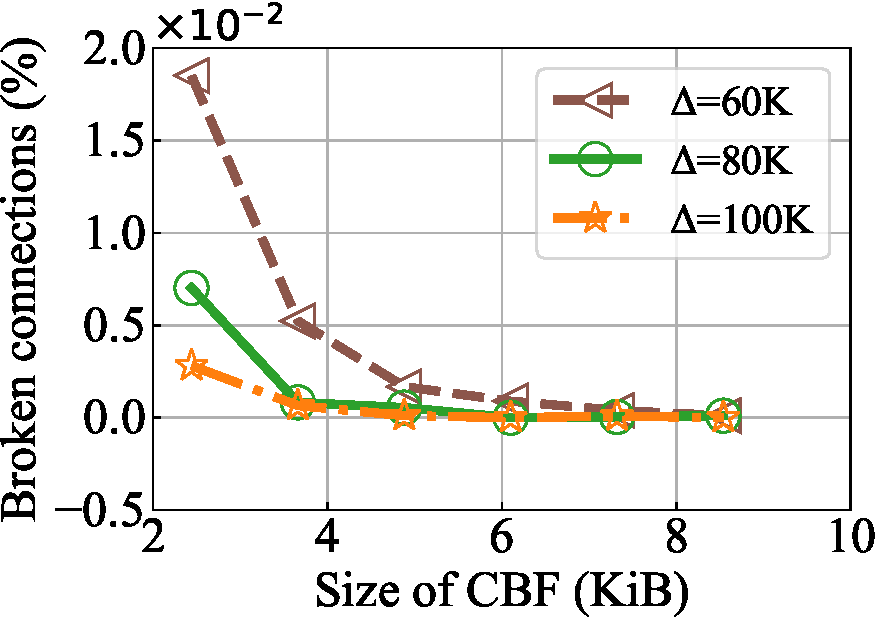
\includegraphics[width=1\linewidth]{experiment/5maatbrokenconn131072wb.pdf}
 		\end{minipage}
 		\label{10.1}
 	}
 	\subfigure[Data Mining.]{
 		\begin{minipage}{0.46\linewidth}
 			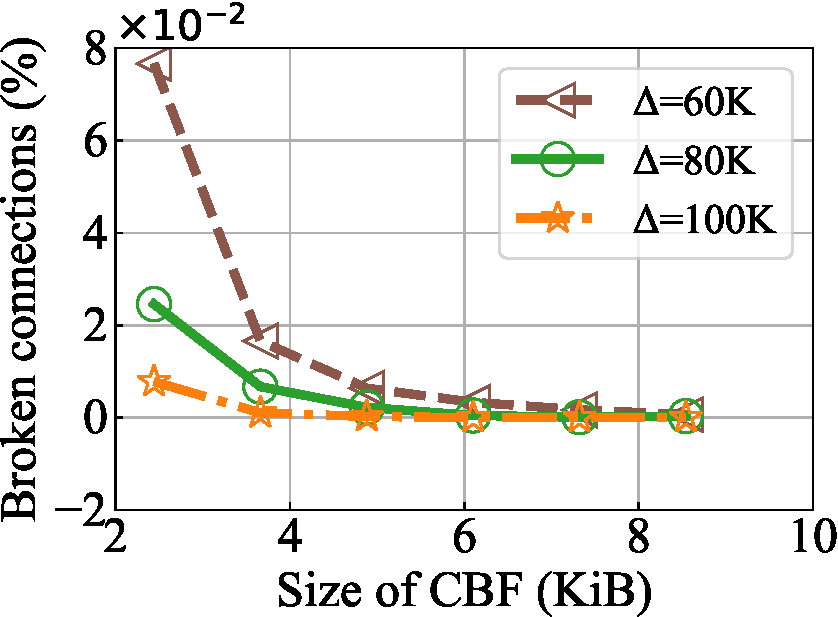
\includegraphics[width=0.98\linewidth]{experiment/5maatbrokenconn131072dm.pdf}
 		\end{minipage}
 		\label{10.2}
 	}
 	\caption{Broken connections ratio for the increasing size of CBF (2.44 KiB$\sim$8.54 KiB).}
 	\label{10}
 \end{figure}

\begin{figure}[t]
	\setlength{\abovecaptionskip}{0pt}
	\setlength{\belowcaptionskip}{-10pt}
	\centering
	\begin{minipage}{0.49\linewidth}
		\centering
		% height=1.8in, width=1.8in
		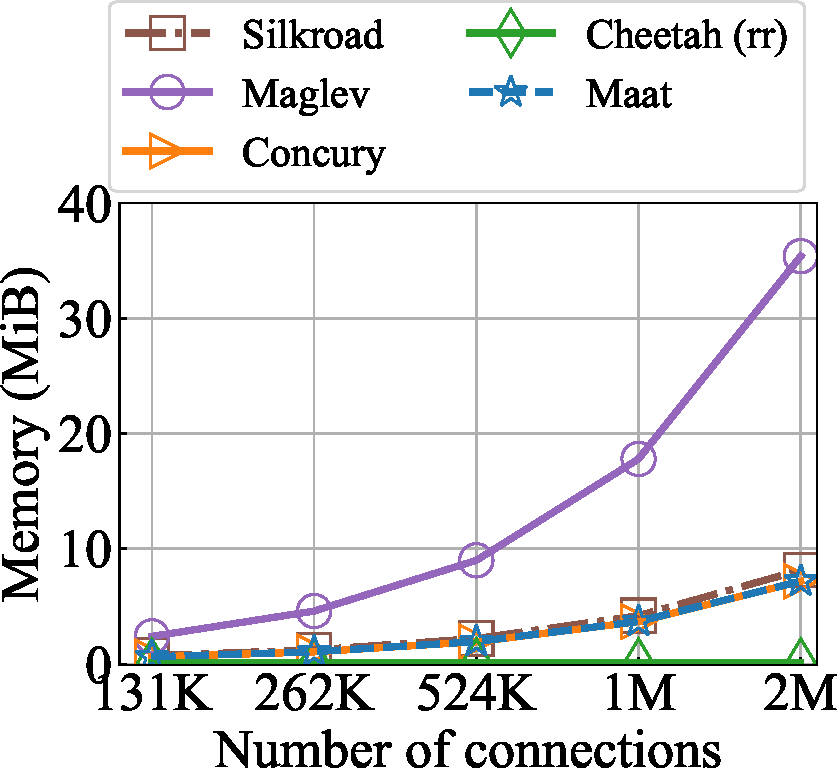
\includegraphics[width=1\linewidth]{experiment/6maatmemory.pdf}
		\caption{Memory cost of various schemes.}
		\label{11}%文中引用该图片代号
	\end{minipage}
	%\qquad
	\begin{minipage}{0.49\linewidth}
		\centering
		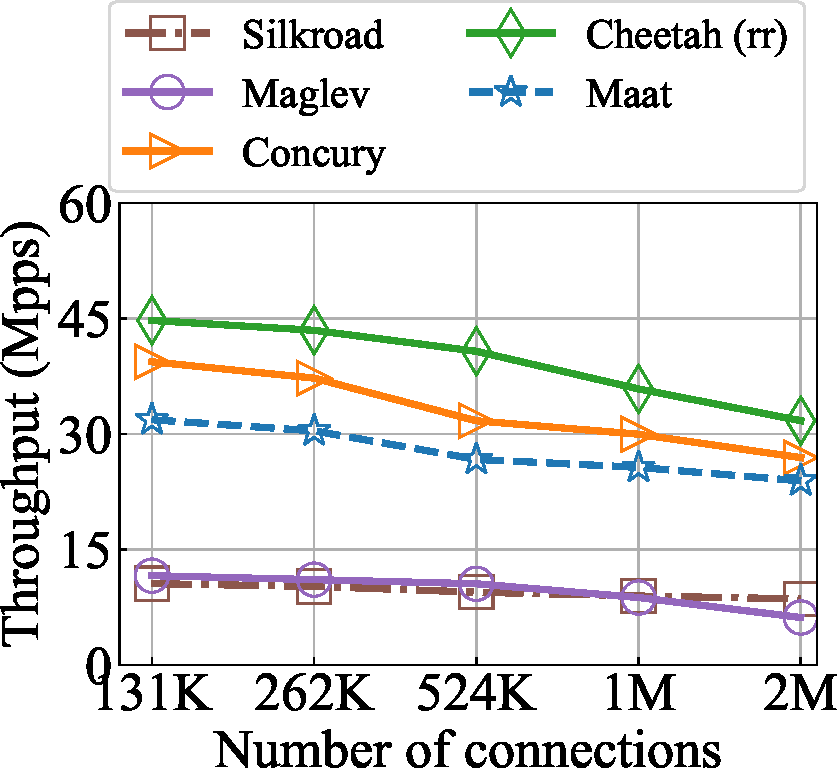
\includegraphics[width=1\linewidth]{experiment/7maatprocess.pdf}
		\caption{Process throughput of various schemes.}
		\label{12}%文中引用该图片代号
	\end{minipage}
\end{figure}

\textbf{PCC Violations under the different workload.} Avoiding PCC violations is a key feature of L4 LB. Maat does not experience broken connections when the DIP pool updates, but the power of one random choice brings potential broken connections. We solve this problem using CBF. Therefore, we evaluated the memory overhead required by CBF to fully guarantee PCC under heavy load (130K connections) before the next data plane update. The results are shown in Fig. \ref{10}. When $\Delta$ is 100K packets, CBF only needs 5.6 KiB memory overhead to fully guarantee PCC under both workloads. The main reason is that in Maat, only a small part of traffic (1.59\%) requires CBF insertion. For modern servers, a few KiB of memory overhead is negligible. Table II shows the PCC violations of several existing typical LB schemes \cite{barbette2021cheetah, shi2020concury}. Similar to Concury and Cheetah, Maat can guarantee 100\% PCC when sufficient memory resources are provided. However, Concury struggles to achieve better fairness, while Cheetah requires modifications to the existing protocol stack.

\begin{table}[htbp]
	\centering
	\caption{Broken connections ratio of various schemes.}
	\begin{tabular}{|c|c|} %l(left)居左显示 r(right)居右显示 c居中显示
		\hline 
		Schemes&Broken connections\\
		\hline  
		Hash (\cite{patel2013ananta, gandhi2015rubik})&11\%\\
		\hline
		Consistent-Hash (\cite{eisenbud2016maglev})&3\%\\
		\hline
		Concury (\cite{shi2020concury})&0\%\\
		\hline
		Cheetah (\cite{barbette2021cheetah})&0\%\\
		\hline
		Maat&0\%$\sim$0.0766\%\\
		\hline
	\end{tabular}
	\label{1}
	\vspace{0em}
\end{table}

\begin{figure*}[h]
	\setlength{\abovecaptionskip}{0pt}
	\setlength{\belowcaptionskip}{-10pt}
	%  for a heavy-tailed workload.
	\centering
	\begin{minipage}{0.245\textwidth}
		\centering
		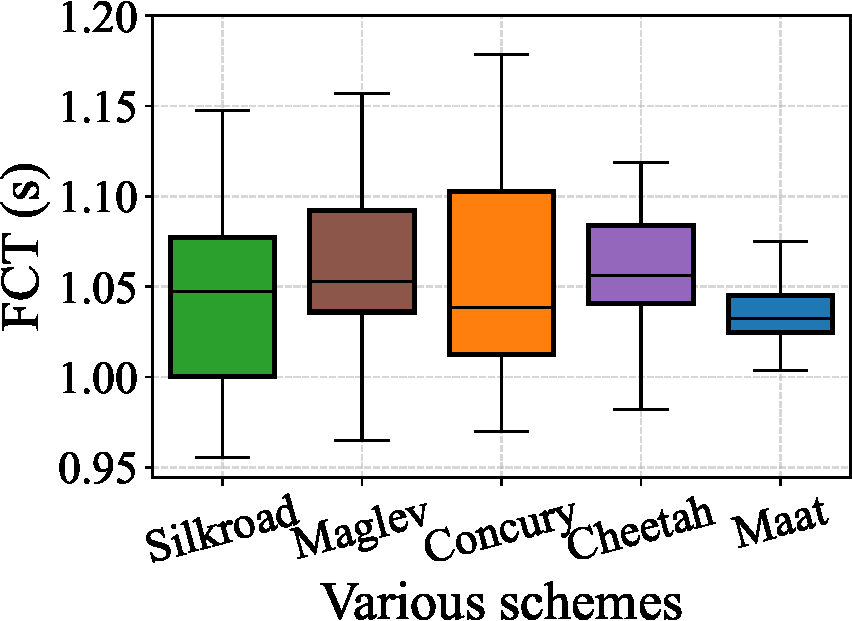
\includegraphics[width=1\textwidth]{experiment/8boxplotfct.pdf}
		\caption{Evaluation of various L4 LB schemes.}
		\label{13}
	\end{minipage}
	%\qquad
	\begin{minipage}{0.245\textwidth}
		\centering
		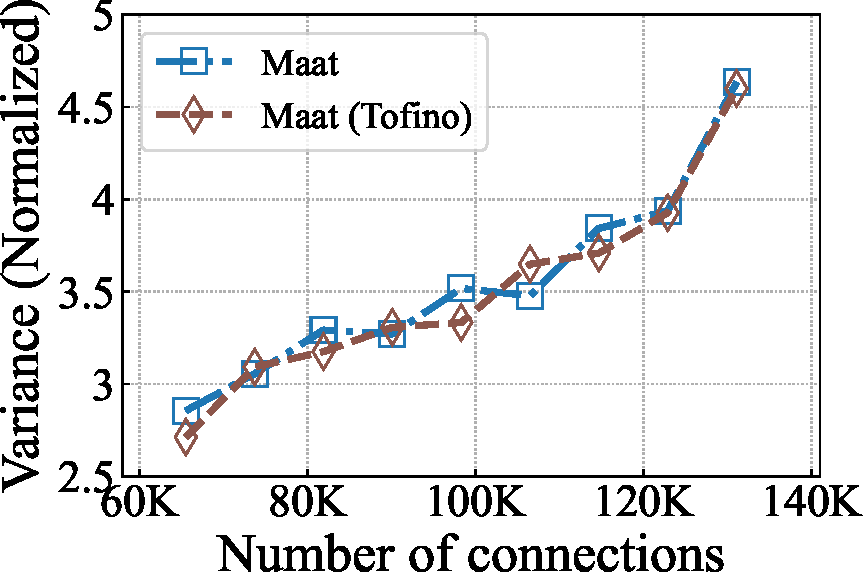
\includegraphics[width=1\textwidth]{experiment/9var.pdf}
		\caption{Variance of Maat and Maat (Tofino).}
		\label{14}
	\end{minipage}
	\begin{minipage}{0.245\textwidth}
		\centering
		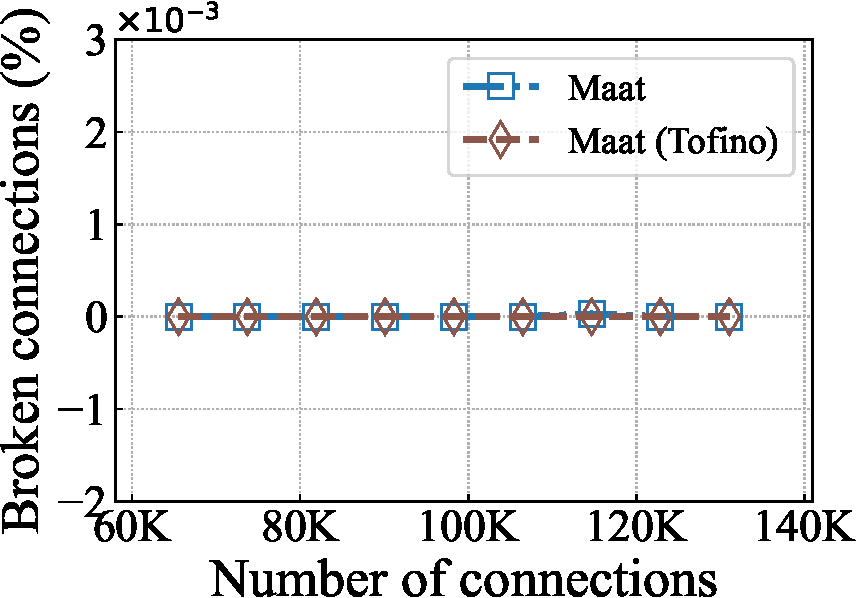
\includegraphics[width=1\textwidth]{experiment/10broken.pdf}
		\caption{Broken connections ratio of Maat and Maat (Tofino).}
		\label{15}
	\end{minipage}
	\begin{minipage}{0.245\textwidth}
		\centering
		% height=1.5in, width=1.8in
		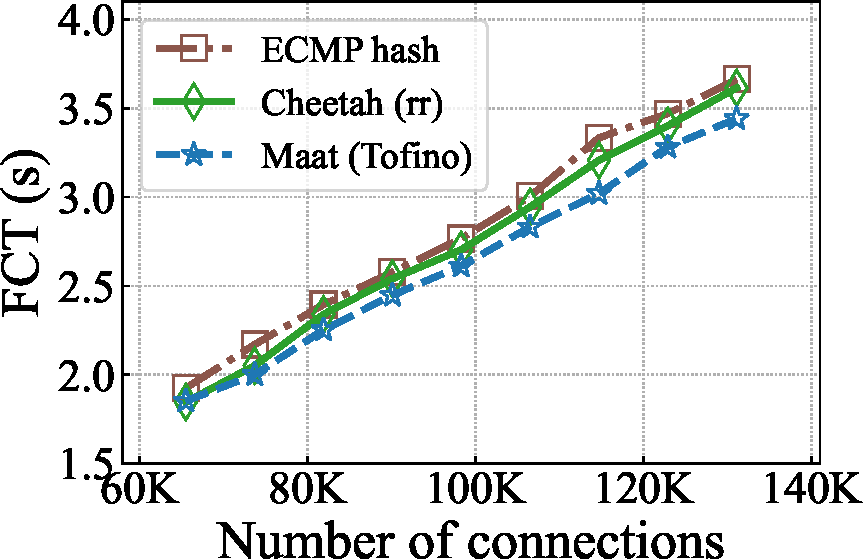
\includegraphics[width=1\textwidth]{experiment/11tofinofct.pdf}
		\caption{Flow completion time for Tofino experiment.}
		\label{16}
	\end{minipage}
\end{figure*}

\subsection{Evaluation of DPDK implementation}
Maat runs on a dual-socket Intel Xeon Silver 4210R CPU @ 2.40GHz, with a total of 40 logical CPU cores (10 cores per socket). We implement Maat using the Data Plane Development Kit (DPDK), a series of libraries for fast user-space packet processing \cite{pktgenDPDK}. In this testbed, we connect two commodity servers (\emph{S1} and \emph{S2}) to the Maat, and the configuration information is the same as the server where Maat is located. The Servers are connected via 100G Mellanox Connect-X 5 NICs. Logically, \emph{S1} acts as a client and \emph{S2} emulates 32 backend servers (DIPs). To evaluate the memory overhead and processing throughput of LB, we use Pktgen-DPDK \cite{pktgenDPDK} on the \emph{S1} to generate traffic and send them to the \emph{S2} through the LB. To evaluate flow completion time, we generated HTTP requests through WRK on \emph{S1}, and each core of \emph{S2} performs a constant amount of CPU-intensive work to schedule the 8KB file \cite{barbette2020high}.

\textbf{Memory Usage.} Fig. \ref{11} shows the memory cost required to store different connections for Maglev, SilkRoad, Concury, Cheetah, and Maat respectively. Cheetah does not need to maintain the mapping relationship between connections and servers as it stores the DIP in the packet header. Therefore, the memory resources occupied by Cheetah do not increase as the number of connections increases. To maintain PCC, the remaining schemes need to maintain the mapping relationship between connections and DIPs on LBs. As the number of connections increased, we found that the memory cost of Maglev is 79.75\% higher than the other three schemes. SilkRoad, Concury, and Maat occupy similar storage spaces. Compared with Concury, Maat introduces the following additional memory overhead: 1) State information about the DIPs needed to improve fairness; 2) CBF. When the number of connections is 1.04 million, the Maat additional overhead only accounts for 0.18\% of the total overhead. However, it can fully guarantee PCC and improve fairness by about 70\%.

\textbf{Process Throughput.} We also investigated the processing throughput of different L4 LB schemes. The higher the processing throughput, the fewer LBs we need to deploy. In this experiment, the metric is millions of packets per second (Mpps). In Fig. \ref{12}, we found that Cheetah (rr) has a 24.63\% improvement over Maat because it does not need to perform operations such as inserting and querying table entries in LB. However, it cannot be ignored that the actual deployment of Cheetah requires modification of the protocol stack. In contrast, Maat is easy to implement without any changes to end-hosts or protocol stack, and can be incrementally deployed in existing networks. Compared with Concury, the throughput of Maat is reduced by 14.01\% due to additional compute-intensive operations required to improve the fairness of server loads. However, compared with Maglev and Silkroad, Maat's operations on the data plane are simpler, resulting in improvements of 65.09\% and 60.5\%, respectively.

\textbf{Maat improves flow completion time with heavy-tailed workloads.} Fig. \ref{13} shows the distribution of flow completion times for 32 servers. \emph{S1} uses WRK to generate heavy-tail distributed HTTP requests (130K connections). For Maglev, Silkroad, and Concury, we find that some servers in these three schemes have high FCT, which verifies that hash-based LB has poor fairness performance as mentioned above, while the FCT of Maat is improved by up to 10.58\% compared to these solutions. Compared with these hash-based schemes, the improvement of Cheetah (rr) is not significant, because under heavy-tailed distribution, some servers are loaded unpredictably, and Cheetah (rr) struggles to cope with this scenario. This experiment demonstrates the advancement of the scheduling method (power of one random choice) used in Maat, which can help us make full use of the resources of all servers.

\begin{table}[tbp]
	\centering
	\caption{Resource consumption of Maat and Cheetah (rr).}
	\begin{tabular}{|c|c|c|} %l(left)居左显示 r(right)居右显示 c居中显示
		\hline 
		Resource&Maat&Cheetah (rr)\\
		\hline  
		Hash Bits&3.8\%&2.1\%\\
		\hline
		Gateway &8.3\%&4.2\%\\
		\hline
		SRAM &2.2\%&1.8\%\\
		\hline
		VLIW Actions&6.0\%&2.6\%\\
		\hline
		ALU Instruction&12.5\%&4.2\%\\
		\hline
	\end{tabular}
	\label{1}
	\vspace{-1em}
\end{table}

\subsection{Evaluation of Tofino implementation}
We implemented Maat on the Tofino target, where the data plane contains about 700 lines of P4 code. Due to the limitation of hardware resources that are exclusively accessed at all stages of the pipeline, we did not count the first packet of each flow, but this did not affect our measurement of the load on different servers. In Fig. \ref{14} and Fig. \ref{15}, we compare the hardware implementation (Maat (Tofino)) and the ideal implementation (Maat), and we can find that our compromised implementation on the Tofino switch does not affect the improvement of fairness and the maintenance of PCC. We use thrift to implement communication between the data plane and the control plane. Once a DIP pool update event occurs, the ASDP needs to be changed, which is done by the control plane through the thrift API. Maat also uses the thrift API to clear the CBF and update the DIP_table to forward new connections to the correct DIP. In this experiment, we use the WRK HTTP request generator on one machine as the client and 32 cores of another machine as the 32 servers, where the two servers are connected through a Tofino switch.

Maat is compared with the following two methods in this experiment: 1) a simple hash-based LB implemented in P4; 2) stateless Cheetah using round-robin (rr), with an increasing number of connections for 1MB files. Table III shows the hardware resource usage of the packet processing pipeline at the programmable switch under Maat and Cheetah (rr). Maat uses more matching action tables and stages in the pipeline to implement comparison and calculation logic. These operations require more stateful ALU and SRAM, resulting in higher consumption of resources such as gateway, SRAM, and ALU instructions. In short, compared to Cheetah (rr), Maat consumes more hardware resources due to fine-grained scheduling of incoming traffic. However, the limited resource consumption is acceptable compared to the benefits of load balancing. In Fig. \ref{16}, we observe that FCT of Maat has a 9.67\% improvement compared to hash-based LB and still a 6.01\% improvement compared to Cheetah with round-robin. Maat achieves better FCT under higher loads because it takes advantage of the opportunities brought by random selection to more fully utilize all available server resources.